% chktex-file 44
\chapter{Spesifikasi Kebutuhan Perangkat Lunak}

\section{Pendahuluan}

\subsection{Tujuan Penulisan Dokumen}

Dokumen berikut ditulis untuk menggambarkan spesifikasi kakas untuk tugas akhir yang berjudul ``\thesistitle''.
Dokumen ini akan menjelaskan secara ringkas pemodelan implementasi dari kakas yang hendak dirancang.
Dokumen ini bertujuan untuk membantu penulis tugas akhir dalam memodelkan kakas serta membantu penulis dalam proses implementasi kakas.

\subsection{Lingkup Masalah}

Pengembangan sistem pemelajaran mesin tidak terlepas dari otomatisasi pada sistem pada umumnya.
Kakas bertujuan untuk membantu proses otomatisasi dalam pembangunan sistem pemelajaran mesin.
Otomatisasi yang dilakukan akan membantu proses pembangunan sistem pemelajaran mesin dalam hal membentuk kode-kode yang diperlukan.
Kode-kode yang diperlukan merujuk pada kode yang dibutuhkan sistem untuk dapat dilakukan inferensi terhadap model dari pihak luar.

\subsection{Definisi, Istilah  dan Singkatan}

Bagian ini akan menuliskan beberapa hal yang memiliki domain yang spesifik terkait pada pengembangan kakas ini.
Berikut ini adalah beberapa definisi, istilah, dan singkatan yang tertulis dalam dokumen ini.

\begin{itemize}
    \item \textbf{Kakas}: mendefinisikan suatu jenis perangkat lunak yang digunakan untuk membantu suatu proses.
    \item \textbf{Sistem}: mendefinisikan suatu jenis perangkat lunak yang memiliki \textit{interface} tertentu untuk melakukan suatu perintah untuk melakukan perubahan dalam sistem atau menghasilkan suatu keluaran yang dapat digunakan oleh sistem.
    \item \textbf{Pemelajaran Mesin}: dikenal juga sebagai \textit{machine learning}, suatu teknik untuk menghasilkan prediksi berdasarkan data yang diberikan kepada program yang berdasarkan pada teknik optimasi.
    \item \textbf{Eksperimen}: dalam dokumen ini, konteks eksperimen adalah kepada eksperimen pemelajaran mesin atau proses pelatihan serta evaluasi model.
    \item \textbf{Sistem Pemelajaran Mesin}: perangkat lunak yang menerima perintah berupa masukan data yang kemudian akan dihasilkan prediksi menggunakan model pemelajaran mesin, di mana prediksi tersebut dikembalikan melalui sistem.
    \item \textbf{CLI}: merupakan singkatan dari \textit{command-line interface} yang adalah salah satu jenis tampilan antarmuka yang memanfaatkan terminal atau \textit{command line} untuk berinteraksi dengan pihak eksternal.
\end{itemize}

\subsection{Aturan Penomoran}

Berikut ini adalah daftar beberapa aturan penomoran yang terdapat dalam dokumen ini.
\begin{itemize}
    \item \textbf{FRXXX}: menyimbolkan kebutuhan fungsional ke-XXX.
    \item \textbf{NFRXXX}: menyimbolkan kebutuhan non-fungsional ke-XXX.
\end{itemize}

\subsection{Ikthisar Dokumen}

Bagian pertama dokumen ini akan membahas pendahuluan mengenai kepentingan, fungsi, serta aturan yang terdapat dalam dokumen ini.
Bagian kedua dokumen ini mendefinisikan penjelasan secara umum mengenai kakas.
Bagian ketiga dokumen ini mengenumerasikan dan menjelaskan spesifikasi kebutuhan untuk kakas ini, baik secara fungsionalitas atau dari sisi pengguna.

\section{Deskripsi Umum Perangkat Lunak}

\subsection{Deskripsi Umum Kakas}

\begin{figure}[ht]
    \centering
    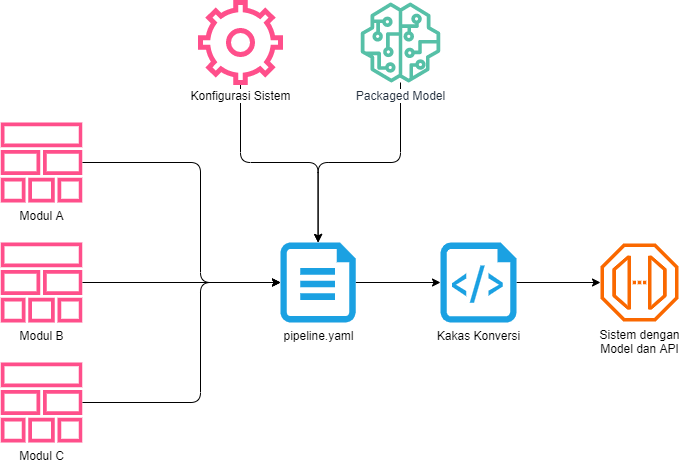
\includegraphics[width=0.7\textwidth]{03-rancangan-solusi.drawio.png}
    \caption{Gambaran Umum Alur Penggunaan Kakas}\label{fig:appendix-tool-design}
\end{figure}

Kakas ini merupakan kakas yang melakukan otomatisasi pada tahapan pembentukan kode untuk sistem.
Secara umum, kakas ini akan menerima masukan berupa \textit{file-file} yang dihasilkan pada tahapan eksperimen.
\textit{File-file} eksperimen yang dihasilkan merujuk kepada model pemelajaran mesin serta \textit{file-file} lainnya yang diperlukan untuk melakukan pemrosesan data.
Hasil sistem yang akan dibentuk tercatat dalam sebuah \textit{file} konfigurasi.

Konfigurasi kakas terdiri atas lima bagian utama, yaitu sebagai berikut:

\begin{enumerate}
	\item Konfigurasi masukan, yaitu bagian yang mengatur bentuk masukan terhadap sistem.
	\item Konfigurasi keluaran, yaitu bagian yang mengatur bentuk keluaran sistem yang juga merupakan hasil prediksi model.
	\item Konfigurasi model, yaitu bagian yang mengatur format model serta letak model.
	\item Konfigurasi pemrosesan data, yaitu bagian yang mengatur kode pemrosesan data terhadap masukan sistem untuk melakukan pemetaan menjadi masukan model.
	\item Konfigurasi \textit{Interface} yang disediakan, yaitu bagian yang mengatur \textit{interface} apa saja yang digunakan oleh sistem untuk melakukan inferensi. 
\end{enumerate}

\subsection{Karakteristik Pengguna}

Pengguna dari kakas ini merupakan pengguna yang sudah lazim dan terbiasa dengan penggunaan CLI dan memiliki pemahaman terhadap .
Bila dilihat dari sisi peran dalam sebuah tim pengembang sistem, kakas ini ditujukan pada pengguna yang berperan dalam eksperimen pemelajaran mesin serta yang berperan dalam pengimplementasian sistem pemelajaran mesin.
Untuk pengembangan awal kakas, saat ini kakas lebih ditujukan pada pengguna yang hendak melakukan \textit{prototyping} kepada sebuah sistem pemelajaran mesin.

\subsection{Batasan}

Terdapat batasan implementasi untuk kakas ini untuk menyesuaikan dengan tujuan kakas yang ditujukan sebagai \textit{proof-of-concept}.
Berikut adalah beberapa batasan dari sisi implementasi kakas:

\begin{itemize}
    \item Eksperimen pemelajaran mesin terbatas untuk eksperimen dengan permasalahan yang \textit{supervised} saja.
    \item Kakas dibatasi untuk menghasilkan sistem yang \textit{REST-like} saja sebagai contoh.
    \item Keluaran dari kakas hanya perlu dapat mengembalikan prediksi saja.
\end{itemize}

\subsection{Lingkungan Operasi}

Implementasi kakas dilakukan menggunakan bahasa Go 1.18 yang dapat menghasilkan kode Python 3.
Untuk menjalankan kakas diperlukan Python dan Pip dengan versi yang bersesuaian.
Kedua hal tersebut diperlukan karena kakas ini juga sekaligus akan melakukan instalasi terhadap \textit{library-library} yang diperlukan oleh sistem.
\textit{Library} tersebut akan diinstalasikan dalam sebuah \textit{virtual environment}, sehingga \textit{package-package} terkait perlu diunduh juga untuk dapat menggunakan \textit{virtual environement} tersebut.
Untuk konfigurasi dari kakas, akan digunakan suatu format data yang dapat menyimpan informasi secara terstruktur.
Kakas ini diimplementasikan untuk dapat menerima konfigurasi berbentuk YAML.

Kakas ini akan diimplementasikan dan dijalankan pada lingkungan berbasis pada kernel Linux.
Pengujian terhadap kakas juga akan dilakukan pada lingkungan berbasis Linux menggunakan distribusi sistem operasi Ubuntu 20.04.
Implementasi kakas ini yang menggunakan bahasa Go tidak menutup kemungkinan bahwa kakas ini dapat dijalankan pada sistem operasi lain, namun untuk pengujian dan implementasi ditetapkan hanya untuk sistem operasi tersebut.

\section{Deskripsi Kebutuhan}

\subsection{Kebutuhan Antarmuka Eksternal}

Bagian ini akan mencatat beberapa hal mengenai kebutuhan antarmuka kakas.
Kebutuhan antarmuka meliputi pihak eksternal yang berhubungan dengan kakas agar kakas dapat berjalan sesuai spesifikasi yang ditetapkan.

\subsubsection{Antarmuka Perangkat Lunak}

Seperti yang telah disinggung sebelumnya, kakas ini memerlukan Python untuk menjalankan beberapa hal.
Python akan menjadi antarmuka untuk kakas ini untuk melakukan hal tersebut.
Pip yang juga merupakan bagian dari Python untuk melakukan pengunduhan dan instalasi \textit{library} juga diperlukan sebagai antarmuka. 

\subsubsection{Antarmuka Komunikasi}

Keperluan kakas untuk melakukan pengunduhan dan instalasi mengharuskan kakas terhubung dengan koneksi internet.
Tanpa koneksi internet, kakas tidak akan berjalan dengan benar.
Kakas tidak menyediakan \textit{caching} untuk \textit{library-library} yang diunduh.

\subsection{Kebutuhan Fungsional}

\begin{table}
    \small
    \caption{Daftar Kebutuhan Fungsional Kakas}\label{table:functional-req}
    \begin{center}
        \begin{tabular}{|p{0.1\linewidth} | p{0.4\linewidth} | p{0.5\linewidth}|} 
            \hline
            \textbf{ID} & \textbf{Kebutuhan} & \textbf{Penjelasan}\\ [0.5ex] 
            \hline
            FR001 & Kakas dapat membaca konfigurasi dengan format tertentu. & Konfigurasi dibaca untuk memetakan hasil akhir sistem buatan kakas. \\ 
            \hline
            FR002 & Kakas dapat XXX & XXX \\ 
            \hline
            FR003 & Kakas dapat XXX & XXX \\ 
            \hline
        \end{tabular}
    \end{center}
\end{table}

\subsection{Kebutuhan Non Fungsional}

\subsection{Lingkungan Operasi}


